\documentclass[10pt]{article}
\usepackage{comment}
\usepackage{listings}
\usepackage{graphicx}
\usepackage{psfrag}
\usepackage{amssymb}
\usepackage{amsmath}
\usepackage{algorithm2e}
\usepackage{caption}
\usepackage{epstopdf}
\usepackage{url}
\usepackage{fullpage}

\usepackage{float}
\floatplacement{figure}{H}

%\usepackage{epsfig}

\begin{comment}
\newtheorem{theorem}{Theorem}[section]
\newtheorem{proposition}[theorem]{Proposition}
\newtheorem{lemma}[theorem]{Lemma}
\newtheorem{corollary}[theorem]{Corollary}
\newtheorem{definition}[theorem]{Definition}
\end{comment}

\usepackage{enumerate}

%\usepackage{psfrag}

\usepackage{subfigure}

%\usepackage{graphicx}
%\usepackage{caption}
%\usepackage{subcaption}

\usepackage{epsfig}

\usepackage{color}% Include colors for document elements (required for psfrag)
\usepackage{psfrag}

\newcommand{\psdir}{./sections}
\newcommand{\ldir}{./sections}
\newcommand{\fig}{./sections/fig}
\newcommand{\comm}[1]{}


\def\IL{{\it left}}
\def\IM{{\it middle}}
\def\IR{{\it right}}
\def\IB{{\it bottom}}
\def\IT{{\it top}}


\newcommand{\algref}[1]{Algorithm~\ref{#1}}
\newcommand{\defref}[1]{Definition~\ref{#1}}
\newcommand{\secref}[1]{Section~\ref{#1}}
\newcommand{\figref}[1]{Figure~\ref{#1}}
\newcommand{\tabref}[1]{Table~\ref{#1}}
\newcommand{\thmref}[1]{Theorem~\ref{#1}}
\newcommand{\propref}[1]{Proposition~\ref{#1}}
\newcommand{\efct}[1]{$\langle$ #1 $\rangle$}

\newcommand{\chapref}[1]{Chapter~\ref{#1}}



\newcommand{\atlasMgrid}{Atlas MultiGrid}
\newcommand{\cg}{$\cal{G}$}
\newcommand{\cgraph}{active constraint graph}
\newcommand{\sgraph}{stratification graph}
\newcommand{\cs}{$\cal{S}$}
\newcommand{\cd}{colldet}
\newcommand{\pconfig}{parametrized configuration}
\newcommand{\orient}{pose}
\newcommand{\point}{point}
\newcommand{\helix}{molecular composite}
\newcommand{\atom}{atom marker}
\newcommand{\dumbell}{dumbell}
\newcommand{\EASAL}{\texttt{EASAL}}
\newcommand{\Cr}{Cartesian realization}

\newcommand{\tns}{T} %total number of samples
\newcommand{\C}{C} %the collection of interesting atom pairs
\newcommand{\m}{m} %size of S
\newcommand{\stp}{s}


\newcommand{\tol}{$\tau$}
\newcommand{\AC}{A}
\newcommand{\mU}{M}
\newcommand{\aU}{atom marker}
\newcommand{\acg}{G}

\newcommand{\cover}{boundaries}


\newcommand{\aview}{atlas view}
\newcommand{\pview}{parametrized chart view}
\newcommand{\rview}{realization view} %configuration space view
\newcommand{\param}{parameter}
\newcommand{\idialog}{intervention dialog}
\newcommand{\ndialog}{node selection dialog}
\newcommand{\atlas}{atlas}
\newcommand{\threeRealizable}{$3$-realizable}
\newcommand{\chart}{chart}

% for lists
\renewcommand{\labelitemi}{$\bullet$}



\def\jorg#1{\textcolor{blue}{#1}}
% \def\aysegul#1{\textcolor{red}{#1}}
\def\mred#1{\textcolor{red}{#1}}


% for review
\definecolor{seagreen}{RGB}{48,178,139}
\definecolor{yelloworange}{RGB}{249,146,0}
\definecolor{plum}{RGB}{127,0,126}

\newcommand{\aysegul}[1]{{\color{blue}#1}}
\newcommand{\meera}[1]{{\color{magenta}#1}}
\newcommand{\troy}[1]{{\color{seagreen}#1}}
\newcommand{\rahul}[1]{{\color{cyan}#1}}
\newcommand{\joel}[1]{{\color{yelloworange}#1}}
\newcommand{\ruijin}[1]{{\color{plum}#1}}


%opening
\title{EASAL User/Developer Manual}

\author{Aysegul Ozkan, Rahul Prabhu, Troy Baker, \\James Pence, Jorg
Peters, Meera Sitharam \\ University of Florida}

 
\begin{document}

\maketitle
This is a user/developer guide for the EASAL software described in the
accompanying TOMS paper.
EASAL generates, describes the topology, and explores the configuration space 
of two point sets in $\mathbb{R}^3$ that are mutually constrained by
distance intervals. Technical concepts and definitions that are required to use
this software can be found in the main paper.


\section{Introduction}
\label{sec:intro}
EASAL generates the assembly configuration space of two point sets in $\mathbb{R}^3$
and describes the key aspects of the topology and geometry of of this space
~\cite{Sitharam:2012:EASAL, Ozkan2014MainEasal, Wu2014Virus}.
EASAL implements
algorithms that use new theoretical results, some of which are presented in
~\cite{Ozkan2014MainEasal, SiGa:2010, Sitharam:2012:EASAL}.  
EASAL is opensource and can be downloaded from
\url{https://www.bitbucket.org/geoplexity/EASAL}.  

This user guide describes the TOMS version of EASAL.
The TOMS version is the backend of EASAL
without the GUI and with text input and output. Only this version of
EASAL is part of the TOMS submission. 
The experimental results in Section 4.1 of the paper can be reproduced
with this version using the sample input files given in the files directory 
(see Section \ref{sec:test} for instructions).


This user guide describes in depth the key conceptual functionalities,
dependencies and installation, and the major classes and methods in EASAL.  
A video presenting the theory, applications, and software components of
EASAL is available at \url{http://www.cise.ufl.edu/~rprabhu/EASALvideo.mpg}.

An optional GUI (not part of TOMS submission) has been included for intuitive
visual verification of the results.  Instructions on how to install, how to use
and major functionalities offered by the GUI have been detailed in the
`Complete User Guide'. The source code and the `Complete User Guide' are
present in the EASAL github respository which can be found at
\url{https://www.bitbucket.org/geoplexity/EASAL}.\\ 


\noindent\textbf{Organization:} 
The rest of the user guide is organized as follows.
Section \ref{sec:dependency} discusses the software dependencies and
installation instructions, Section \ref{sec:io} discusses the input and output,
Section \ref{sec:functionalities} discusses the functionalities offered by the
backend. Section \ref{sec:test} gives an example test driver and Section
\ref{sec:classes} describes the major classes and methods in EASAL to help
developers gain an insight into how EASAL has been implemented.

\section{Dependencies and installation}
\label{sec:dependency}
\subsection{Dependencies}
This section discusses the software dependencies of EASAL and gives installation instructions.

\begin{itemize} 
  \item Operating System: EASAL has been tested only on the following platforms:
	\begin{itemize}
	\item Ubuntu 12.04 or higher.
	\item Fedora 22 or higher.
	\item OS X 10.8 Mountain Lion.
	\end{itemize}
	  EASAL should work on any UNIX variant platform with little to no modifications.

  \item We use Version 2.0 of the \emph{Eigen} library for linear algebra
		  computations. All necessary files pertaining to Eigen required by
		  EASAL are provided with the source code in the \emph{include}
		  directory.  
   
  \item We use \emph{simpleini} to read the settings from the
		  settings.ini file. All necessary files pertaining to simpleini are
		  provided with the source code in the include directory.
   
  \item C++ compiler: EASAL requires one of the following compilers
		  \begin{itemize}
		  	\item g++ Version 4.8 or higher.
		  	\item clang++ Version 3.8 or higher.
		  \end{itemize}
		  
  \item EASAL uses the GNU Make utility to compile the source files. Make
		  Version 4.1 is required.
\end{itemize}

 
\subsection{Installation}
\label{sec:installation}
\begin{itemize}
	 \item Install GNU Make
	   \begin{itemize}
	   	   \item On Ubuntu 
	   	   \begin{itemize}
			\item sudo apt-get install make
		   \end{itemize}	
		   \item On Fedora
		   \begin{itemize}
			\item yum install make
		   \end{itemize}
		   \item On OSX
		   \begin{itemize}
		   \item sudo xcode-select -switch /Applications/Xcode.app/Contents/Developer
		   \end{itemize}
		   \end{itemize}
	 
	 \item To build the software, run \emph{``make backend"} in the build/root directory.
	 \item To run EASAL run \emph{``bin/EASAL''} in a terminal from the root/build directory.
\end{itemize}% subsubsection  (end)

\emph{Before giving the test driver details in Section \ref{sec:test}, we first describe
the input, output and software functionalities.}

\section{Input/Output}
\label{sec:io}
\subsection{Input}
Input to EASAL is specified using the settings.ini file. The main input features are the following:

\begin{itemize}
\item \textbf{Two rigid point sets}: \emph{[PointSet(A/B)]} 
fields are used to specify the two point sets. The file subfield
points to a file that specifies the input data in the pdb format.
		

\item \textbf{Constraints}:
\begin{itemize}
\item \textbf{Active threshold}: This specifies the range of distances where
constraints are considered active.  This is given as $\lambda*(r_i+r_j) \pm
\delta$.  Here, $\lambda$ is specified by the \emph{activeLowerLambda} subfield
and $\delta$ is specified by the delta text box in the input window. $r_i$ and
$r_j$ are the radii of the spheres in the point sets. 

\item \textbf{Collision threshold}: This is the minimum distance between the
points. This too is given as $\lambda*(r_i+r_j) \pm \delta$.  The subfields
\emph{collisionLambda} and \emph{collisionDelta} specify these values.

\item \textbf{Distance Data}: Only when the constraints between these pairs are
active, are the corresponding configuration space regions explored.

\end{itemize}
\end{itemize}

\subsection{Output}

The following are the output:
\begin{itemize}
\item The \emph{Roadmap}, which stores the atlas, i.e., a topologically
stratified set of sample feasible realizations or configurations of the two
rigid point sets. This can be found in the `RoadMap.txt' file in the data
folder.

\item The \emph{Node} files which contain sampling information, Cayley
parameter values, and realizations of the point sets. Each `Node*.txt' file
contains samples for a particular active constraint region.

\item The \emph{paths} file which contains the one degree of freedom motion
path between all pairs of lowest energy configuration regions. This can be
found in the `paths.txt' file in the data folder.

\item The \emph{path matrix}, which contains a path matrix where the rows and
columns correspond to 0D and 1D nodes. The $\{ij\}^{th}$ entry indicates the
number of paths between nodes $i$ and $j$. This can be found in the
`path\_matrix.txt' file in the data folder.

\end{itemize}

\section{Software Functionalities}
\label{sec:functionalities}
\subsection{Active Constraint Graph} 
The active constraint graph for each node in the atlas can be found in the
`RoadMap.txt' file. This active constraint graph shows only the participating
points from each set. A `c' before two points indicates a constraint and a `p'
indicates a parameter between two points belonging to different sets. It has to
be noted that the points in the same set already form a clique.

\subsection{Finding Boundary Regions} The boundary regions of a particular
node of the atlas can be found in the `Roadmap.txt' file. In terms of the
atlas, it depicts the the ancestors and descendants of that node. Since and
edge in the graph represents boundary relationship, this feature allows us to
inspect the boundary regions of an active constraint region.


\subsection{Finding Paths Between Nodes with 6 Active constraints} The atlas
output by EASAL can be used to generate all the paths between any two active
constraint regions along with their energies. Once the atlas has been
generated, finding paths is extremely fast. In the context of molecular
assembly, the path topology of the configuration space is crucial for
understanding assembly kinetics.

Of particular interest is finding paths between two lowest energy
configurations with 6 active constraints or 0D nodes of the atlas with
effectively rigid configurations. We are mainly interested in paths through
active constraint regions that have 5 or 6 active constraints.
One fewer constraint implies one step higher energy and such paths 
represent a continuous one degree-of-freedom motion.

EASAL finds the shortest paths between all pairs of 0D nodes, if they exist.
EASAL writes this path as a series of nodes to the `paths.txt' file.  Once the
sampling has been completed, EASAL computes the total number of paths of a
particular length between every pair of vertices and writes the entire matrix
to the `path matrix.txt' file. The user can specify lengths by setting the
`path length' parameter in the `settings.ini' file.

\subsection{Sampling Options} 
There are two options available:
\begin{itemize}
\item \textbf{Default}: The default mode of sampling is the auto-solve mode,
which samples the atlas in a depth-first fashion. EASAL generates,
depending on the user input, all possible 4D and 5D root nodes. 
EASAL then recursively samples these nodes till the atlas generation
is complete.

\item \textbf{BFS}: Setting the \emph{breadthFirst} subfield under
`[AtlasBuilding]' to true forces EASAL to explore the atlas in a breadth-first
fashion. Otherwise depth-first is used.

\end{itemize}

\subsection{Dimension of the root node}
By default, the dimension of the root node of the atlas is 5, which means that
the root node has one bond and 5 parameters. The \emph{initialContactGraphs}
option under `[RootNodeCreation]' allows the user to change this and make the
root node a 4D node. With a 4D root node, there are 2 bonds and 4 parameters in
the root node.

\subsection{Step Size}
EASAL uses Cayley grid sampling to sample the Cayley space. The user can
specify this using the \emph{stepSize} option under `[Sampling]' in the
settings file. Another option available to the user is to choose dynamic step
size. This option can be selected by setting the \emph{dynamicStepSizeAmong}
under `[Sampling]' to true. Doing so tells EASAL to run the different dynamic
step size variants of EASAL. Setting \emph{dynamicStepSizeWithin} to 0 runs
EASAL-1, setting it to 2 runs EASAL-2 and setting it to 1 runs EASAL-3.

\section{Test Driver}
\label{sec:test}

To run the software, run the following command from the top directory:
`bin/EASAL -settings $<$settings file name$>$'.  Where $<$settings file name$>$
is the path to the settings.ini file in which the input has been specified. All
input to the backend version of EASAL is specified using this settings.ini text
file.

We have included two example test drivers and all necessary files for the
reviewers to run and test the program. To run these, just run the following
commands from the top directory.\\


`bin/EASAL -settings settings example 1.ini'\\


`bin/EASAL -settings settings example 2.ini'\\

Using the test drivers, the results corresponding to `Atlasing and Paths' 
(Section 4.1 in the accompanying TOMS paper) can be
reproduced. The `settings example 1.ini' test driver runs the experiment with n
= 6 example with step set to 0.5 times the smallest radius and the tolerance
set to (1.0 - 0.75) * sum of radii. This corresponds to the third row in Table
I in the TOMS paper. The `settings example 2.ini' runs the experiment with n =
20 with tolerance set to (1.0 - 0.75) * sum of radii and the step size set to
0.25 times the smallest radius. This corresponds to the fourth row in Table I
in the TOMS paper.\\ 


The output of the run can be found in the 'dataDirectory' specified in the
input settings file. For instance, this directory is `Driver1data' for example 1 
and `Driver2data' for example 2. The results are as explained below.


\begin{enumerate}
\item Generating the atlas: The number of samples and the time required for
sampling the entire atlas can be found in the `Samples.txt' file in the data
directory.

\item Finding paths between active constraint regions: As mentioned earlier
EASAL finds the shortest path between all pairs of 0D nodes, if it exists, and
writes this path as a series of nodes to the paths.txt file in the data folder.
Once the sampling has been completed, EASAL computes the total number of paths
of a particular length between every pair of OD regions and writes the entire
matrix to the path matrix.txt file in the data folder. The user can specify
lengths by setting the path length parameter in the settings.ini file. These
results correspond to table II in the TOMS paper.

\item Finding Boundary Regions: The boundary regions of any active constraint
region can be found using the `RoadMap.txt file in the data folder. The `Nodes
this node is connected to' filed in this file lists all the boundary regions.
\end{enumerate}

Sample results for these test drivers have been included in the `SampleOutput'
folder in the top directory.  They contain the following files:
\begin{enumerate}
\item RoadMap.txt - Contains information about the stratification and the
boundary regions.

\item paths.txt - Contains the shortest paths between every pair of 0D nodes,
if it exists.

\item path matrix.txt - Contains the number of paths between 0D and 1D nodes.

\item Samples.txt - Information about number of samples and time required for
sampling.

\item Node0.txt - One typical randomly selected node file containing sampling
information along with realizations.

\end{enumerate}

Once the test drivers have been run, the optional GUI (not part of the TOMS
submission) can be used to visualize the results.  See Section 2.4 of the
complete user guide for instructions on how to visualize the results using the
GUI.  For full use of the GUI, see Section 3 of the `Complete User Guide' which
can be found at \url{https://www.bitbucket.org/geoplexity/EASAL}.  



%WHERE CAN THEY FIND THE COMPLETE USER GUIDE??XXXXXXXXXX

%See Section 3.1 of the complete user guide for the dependencies and installation
%instruction for compiling and running the GUI. To visualize the output of each
%of the drivers, enter the location of the data directory used for each of the
%test drivers in the input window. Click on accept and when prompted to load an
%already sampled atlas, click on yes (See Section 3.3.5 for further details).
%Further GUI functionalities have been described in Section 3.3 and sample GUI
%walkthrough is demonstrated in Section 3.4.


\section{Major Classes of \texttt{EASAL}}
\label{sec:classes}
\begin{figure}[h]
\centering
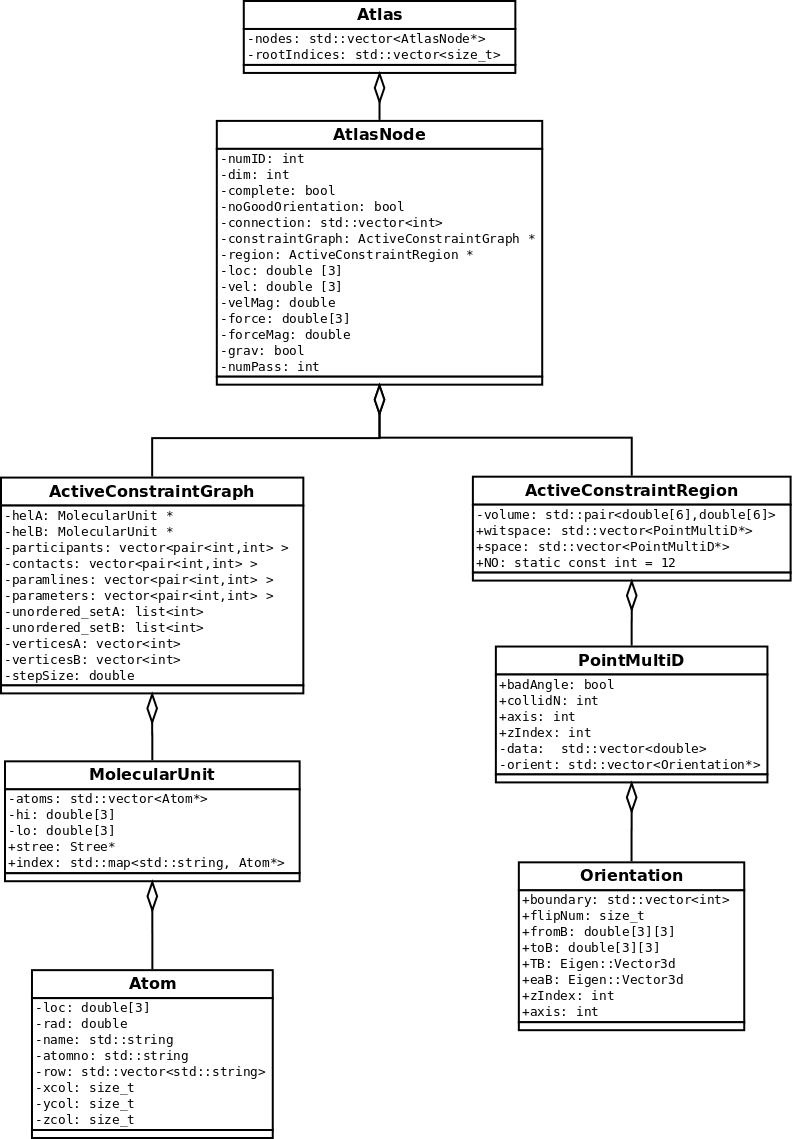
\includegraphics[scale=0.3] {fig/EASAL_UML.png}
\caption{EASAL UML Diagram}
\label{UML}
\end{figure}


\figref{UML} gives an overview of the structure of the major classes of EASAL.
Each of these classes are explained in the subsections below.

\subsection{AtlasBuilder} 

The AtlasBuilder class populates the ActiveConstraintRegion for each
activeConstraintGraph by sampling inside the boundaries of its ConvexChart. 
It creates and explores only regions that contain at least one Cartesian
realization. 

\begin{algorithm} [htbp]
 \SetKwInOut{Input}{input}\SetKwInOut{Output}{output}

 {\bf sampleAtlasNode}\\
 \Input{atlasNode: node}
 \Output{Complete sampling of the atlasNode and all its children}
 \BlankLine
 \LinesNumbered
	$H$ = node.activeConstraints\\
	$G_H$ = node.activeConstraintGraph\\
	\If{ $G_H$ is minimally rigid}
		{stop;	}
	$F$ = complete3Tree($G_H$)\\
	
	$C$ = computeConvexChart($G_H$, $F$)\\

	\For{ each cayleyPoint $p$ within convexChart $C$ }
	{
		$R$ = computeRealizations($p$)\\

		\For{ each realization $r$ in $R$}
		{
			\If{!aPosterioriConstraintViolated($r$)}
			{
				\If{ isBoundaryPoint($r$) \&\& hasNewActiveConstraint($r$, $G_H$) }
				{
					$e$ = newActiveConstraint($r$, $G_H$);\\
					$G'$ := $G_H \cup \{e\}$ ;\\
					\If{ $G'$ is not already present in the current atlas}
					{
						childNode = new atlasNode($G'$)\\
						sampleAtlasNode(childNode);\\
					} \Else{
						childNode = findNode($G'$);
					}
					node.setChildNode(childNode);
				} 
			}
		}
	}

	\caption{High level EASAL pseudocode}
\label{alg:sampleAtlasNode}
\end{algorithm}


\noindent \textbf{Major Attributes:} 
\begin{itemize}
		\item  \textbf{rootGraphs}: The set of all possible 4D or 5D
				ActiveConstraintGraphs of the root nodes
				generated before sampling.
		\item  \textbf{atlas}: An atlas object that is populated by the
				AtlasBuilder by sampling. This object is shared between front-end and
				back-end of the algorithm.
\end{itemize}

\noindent \textbf{Major Methods:}
\begin{itemize}
		\item  \textbf{startAtlasBuilding()}: For each of the generated root graph, 
				creates an atlasNode labeled with a contact graph $G_F$ where $F$ is the
				set of contacts. Then calls the recursive sampleTheNode method 
				for each of the root atlas nodes.
		\item  \textbf{sampleTheNode(atlasNode)}: The exploration of the atlas
				is done by the recursive \textbf{sampleAtlasNode} algorithm (see Algorithm 
				\ref{alg:sampleAtlasNode})
				using one of the generated atlas root nodes as input. This
				algorithm is implemented by the sampleTheNode method. Using
				depth first search this algorithm samples the atlas node and
				all its descendants. 
				
				\textbf{Base case of recursion:} If active constraint graph $G_H$ of the 
				node is minimally rigid i.e., the active constraint region is 
				0-dimensional, we have no more sampling to do, return.
				
				\textbf{The recursion step:} If $G_H$ is not minimally rigid, we use the
				\textbf{complete3Tree} algorithm to find find a set of parameters $F$ so 
				as to form a maximal 3-tree to leverage the convex parametrization theory~
				\cite{SiGa:2010}. This also ensures that $H \cup F$ is minimally rigid and 
				easily realizable. 
				
				The method computeConvexChart shown in the pseudocode finds the convex 
				chart for the parameters $F$ is done by the ConvexChart class explained 
				later. Method ComputeRealizations computes the realization for a 
				Cayley point and is done by the findRealizations method in the software. 
				The aPosterioriConstraintViolated method which checks for angle and steric 
				violations is implemented in the ConstraintCheck class explained later.
				Next we make a call to the findBoundary to detect boundaries and
				newly active constraints.
				

		\item  \textbf{determineStepSizeDynamically()}: Finds out the step size $s$
				given $T$, the total number of samples. Each 5D atlas node has its
				own $s$ computed by using the volume of the Cayley parameter space of the
				node over total number of samples per node. The volume of the
				Cayley parameter space of the node is approximately computed by
				exhaustive sampling within the exact chart without considering
				any constraints. The number of samples per node roughly can be
				computed by $T$ over total number of root(starter) atlas
				nodes, $m$. The number of samples in child nodes are negligible
				since the volume of regions in low dimensional nodes are
				negligible compared to the regions of high dimensional nodes.
		
		\item  \textbf{findBoundary()}: Boundary detection ensures that sampling 
				stays in the feasible region and minimizes discarded samples. 
				The findBoundary method which detects boundary points, checks 
				for newly formed active constraints and makes function calls
				which in turn call sampleTheNode for a child region.
		
\end{itemize}

\subsection{Atlas} 
The `Atlas' class stores the directed acyclic graph that represents the relationship between active constraint regions.

\noindent \textbf{Major Attributes:}
\begin{itemize}
		\item \textbf{nodes}: A vector of all AtlasNodes. 
		\item \textbf{rootIndices}: The indices of all the root nodes in the atlas.
\end{itemize}

\noindent \textbf{Major Methods:}
\begin{itemize}
		\item \textbf{search(node)}: Uses depth first search on the atlas to check
				whether the node exists in the atlas or not. It is used to avoid
				repeated sampling of the same region. The time complexity of
				the search is $O((\text{depth of the tree})) = O(6(k-1)) $ which in our 
				case is $O(1)$ since we fix $k$ to be 2.
\end{itemize}


\subsection{AtlasNode} 
AtlasNodes make up the Atlas. Each AtlasNode represents an active constraint region
reperesented by an ActiveConstraintGraph.

\noindent \textbf{Major Attributes:}
\begin{itemize}
		\item \textbf{acg}: The active constraint graph corresponding to the node.
		\item \textbf{region}: The set of Cayley points in the active region.
		\item \textbf{connection}: The id of the nodes in the atlas that
				represent the boundary of this node's region.
\end{itemize}

\subsection{ActiveConstraintGraph} 
The ActiveConstraintGraph class is used to store the set of active constraints.

\noindent \textbf{Major Attributes:} 
\begin{itemize}
		\item  \textbf{activeConstraints}: The set of point index pairs that represent 
				contacts.
		\item  \textbf{verticesA}: Participating points from first point set.
		\item  \textbf{verticesB}: Participating points from second point set.
		\item  \textbf{parameters}: A vector of point index pairs that represent parameters.
\end{itemize}

\noindent \textbf{Major Methods:}
\begin{itemize}
		\item  \textbf{completeTo3by3Graph()}: Adds points to make sure there
				are at least 3 points from each point set so that the graph is
				realizable. While choosing additional points, it has 2 options,
				choosing the points closest to each other or the points that lead
				to a user specified angle.
\end{itemize}


\subsection{ActiveConstraintRegion} 
The ActiveConstraintRegion class contains the set of feasible Cayley points generated
by sampling.

\noindent \textbf{Major Attributes:} 
\begin{itemize}
		\item  \textbf{space}: The set of feasible Cayley points.
		\item  \textbf{witspace}: The set of feasible witness Cayley points
				obtained from an ancestor node.
\end{itemize}

\noindent \textbf{Major Methods:}
\begin{itemize}
		\item  \textbf{convertSpace(activeConstraintRegion)}: Re-parametrizes
				a region using an input region’s parameters. This method
				converts each Cayley point in the input activeConstraintRegion
				to the Cayley point parametrized by the input region's
				parametrization.
\end{itemize}


\subsection{CayleyPoint} 
The CayleyPoint class represents a multi-dimensional point in the Cayley parameter space
and stores the corresponding Cartesian space orientations of the point set.

\noindent \textbf{Major Attributes:}
\begin{itemize}
		\item  \textbf{data}: Values of the Cayley parameters (non-edge
				lengths). \item  \textbf{orients}: The set of Cartesian space
				Orientations of the point set that were computed by
				realizing the active constraint graph with the given length of
				the edges and non-edges.
\end{itemize}

\subsection{Orientation} 
The Orientation class is the Euclidean transformation of point set. The
Orientation class stores only the information necessary to compute the
transformation matrix that will yield a Cartesian realization for the entire
point set.

\noindent \textbf{Major Attributes:} 
\begin{itemize}
		\item  \textbf{FromB}: Cartesian coordinates of three points from the
				first point set before the transformation.
		\item  \textbf{ToB}: Cartesian coordinates of three points from the
				second point set after the transformation.
		\item  \textbf{connections}: The set of node indices that this
				orientation belongs to. An orientation be on the
				boundary of multiple regions.
\end{itemize}


\subsection{CayleyParameterization} 
The CayleyParameterization class chooses non-edges in an ActiveConstraintGraph
that convert the graph into complete 3-tree. Those non-edges are called the
parameters. The complexity of the sampling algorithm varies based on the
choice of non-edges and the order in which they are fixed.

\noindent \textbf{Major Attributes:} 
\begin{itemize}
		\item  \textbf{partial3tree}: A boolean variable indicating whether
				an ActiveConstraintGraph is partial 3-tree or not.
		\item  \textbf{parameters}: The set of points pairs that represent
				non-edges. 
		\item  \textbf{tetrahedra}: The ordered tetrahedron set that helps in 
				defining the order of parameters that is required
				during the sampling procedure. This data is later passed to
				ConvexChart and CartesianRealizer to help in their computations. 
		\item  \textbf{updateList}: Adjacency map containing the dependency of
				parameters. It provides the set of parameters whose range will
				be updated when one of the parameters is fixed.
		\item  \textbf{boundaryComputationWay}: Inequalities that express the
				range of a parameter can be classified into either a linear or
				non-linear class. This variable is the characterization of the
				parameter that tells what inequality is needed to compute
				the parameter range i.e., triangular or tetrahedral inequality. 
		\item  \textbf{complete3trees}: The set of complete 3 trees.
\end{itemize}

\noindent \textbf{Major Methods:}
\begin{itemize}
		\item  \textbf{defineParameters()}: The parameters of an active
				constraint graph are selected as maximal 3-realizable (3-tree)
				extensions by leveraging the convex parametrization theory.
				\cite{SiGa:2010}. It creates a look-up table containing all possible 
				complete 3-trees. We find a graph in the look-up
				table so that active constraint graph is a proper subset of either the 
				graph or one of its isomorphisms.
		\item  \textbf{parameterMinDeviation()}: An alternate way to pick
				the parameters for 5D regions is by ensuring that the range
				of each parameter is similar. The aim here is to sample more
				uniformly in the Cartesian space. 
		\item  \textbf{built3tree()}: The 3-tree formed by starting with a
				4-vertex complete graph and repeatedly adding vertices in
				such a way that each added vertex is edge-connected to the face
				of a tetrahedron. Store the tetrahedrons in the order they are
				created in the attribute \textbf{tetrahedra}.
\end{itemize}


\subsection{ConvexChart} 

The ConvexChart class is used to determine the \chart\ that parameterize the
regions i.e., it computes the range of parameters of ActiveConstraintGraph. An
exact convex chart yields feasible Cayley points for the current active
constraint region. The resulting Cayley configuration space is convex, before
collisions or other (e.g.\ angle) constraints are introduced. The range of
parameters are computed by triangle and tetrahedral inequalities.

\noindent \textbf{Major Attributes:} 
\begin{itemize}
		\item  \textbf{param\_lengthUpper}: The upper bound of the parameters' range 
		\item  \textbf{param\_lengthLower}: The lower bound of the parameters' range 
		\item  \textbf{param\_length}: current value of parameters
\end{itemize}

\noindent \textbf{Major Methods:}
\begin{itemize}
		\item  \textbf{initializeChart()}: Initalizes the boundaries of
				convex chart. Tighter bounds are given in \cite{ugandhar}. 
		\item  \textbf{computeRange(v1, v2)}: Computes the range of the
				parameter $v1-v2$ in order to eliminate sampling infeasible grid
				points. Range computation is required in every iteration for
				dependent parameters. 
		\item  \textbf{setRangeByTriangleInequality(v1, v2)}: Computes the
				range of the non-edge $v1-v2$ through triangular inequalities.
		\item  \textbf{setRangeByTetrahedralInequality(v1, v2, tetrahedron)}:
				Computes the range of the non-edge $v1-v2$ through tetrahedral
				inequality.
		\item  \textbf{stepGrid}: Sets parameter point to the next grid point
				within the computed range.
		\item  \textbf{stepNeighbour()}: Sets the parameter point to the neighbor
				grid point in all dimensions consecutively.
		\item  \textbf{stepGridBinary()}: Sets the parameter point to 
				somewhere between current point and neighbor grid point
				according to binary search procedure in findBoundary.
\end{itemize}


\subsection{CartesianRealizer} 
The CartesianRealizer class contains routines that
compute orientations that represent transformations of rigid helices
relative to each other. It computes Cartesian realization of an active 
constraint graph with the
parameter lengths taken from cayleyPoint and active constraint lengths for a
specific flip. 
\noindent \textbf{Major Attributes:} 
\begin{itemize}
		\item \textbf{positions}: Cartesian coordinates of vertices in
				ActiveConstraintGraph.
		\item \textbf{edge\_length}: Contains all fixed distances plus current
				distance values of non-edges of ActiveConstraintGraph.
\end{itemize}

\noindent \textbf{Major Methods:}
\begin{itemize}
		\item  \textbf{computeRealization(activeConstraintGraph, convexChart,
				flipno)}: Computes the Orientation by leveraging partial 3-tree
				techniques. activeConstraintGraph which is a complete 3-tree is
				built up from a base tethedra by adding, at each step, a new
				vertex edge-connected to the face of a tetrahedron.
		\item  \textbf{setBaseTetra(tetrahedron)}: Finds Cartesian
				coordinates of the vertices of tetrahedron by known edge
				lengths.
		\item  \textbf{locateVertex(vertex, face)}: Finds Cartesian
				coordinates of the vertex that is connected to the face of a
				tetrahedron.
\end{itemize}


\subsection{ConstraintCheck} 

The ConstraintCheck class is designed to check whether any non-active
constraints become active. Users have the option
to define a set of constraints of interest. In which case, the new constraint
activation check is done only for these. For an input Orientation,
ConstraintCheck first computes the Cartesian realization for the entire \helix\
then passes it to other subroutines to perform user specified constraint check such as
steric constraints or angle constraints.



\bibliographystyle{plain}
\bibliography{easal}

\end{document}
